The dataset used in this study is sourced from TDC NET as a part of a collaboration in connection with this bachelor’s thesis. It consists of hourly time-series measurements collected from 12 cellular network towers across Denmark. The towers are grouped into three categories, urban, recreational, and suburban. The labels are based solely on the geographical location of each tower. Overall summary of the dataset is shown in table \ref{tab:before_pre}. 

\begin{table}[h]
\centering
\caption{Dataset before preprocessing}
\begin{tabular}{lc}
\hline
\textbf{Statistic} & \textbf{After} \\
\hline
Rows & 3,104,976 \\
Urban sites (cells) & 4 (83) \\
Suburban sites (cells) & 4 (93) \\
Recreational sites (cells) & 4 (71) \\
Cells total & 255 \\
Missing rate (data volume dl) & 33.2\% \\
Start date & 2024-05-21 \\
End date & 2026-03-01 \\
\hline
\end{tabular}
\label{tab:before_pre}
\end{table}

The dataset is structured as a multivariate time series. Each row corresponds to an hourly observation, while each column represents a performance indicator describing the network traffic during that hour. Several features are further separated by traffic direction (uplink and downlink). An overview of the features is provided in Table \ref{tab:dataset-features}.

\begin{table}[h]
\centering
\begin{tabular}{lll}
\hline
\textbf{Feature} & \textbf{Type} \\
\hline
Signal-to-noise ratio (SINR max) & continuous \\
Signal-to-noise ratio (SINR avg) & continuous \\
Peak average users & continuous \\
Average users & continuous \\
Peak data volume Downlink & continuous \\
Peak data volume Uplink & continuous \\
Average data volume Downlink & continuous\\
Average data volume Uplink & continuous \\
PRB utilization Downlink & continous \\
PRB utilization Uplink & continuous \\
Average user throughput Downlink & continuous \\
Average user throughput Uplink & continuous \\
Site ID & categorical identifier \\
Cell ID & categorical identifier \\
Frequency technology (4G/5G) & categorical \\
Frequency spectrum & categorical \\
\hline
\end{tabular}
\caption{Overview of dataset features and their types}
\label{tab:dataset-features}
\end{table}

\begin{figure*}[h]
    \centering
    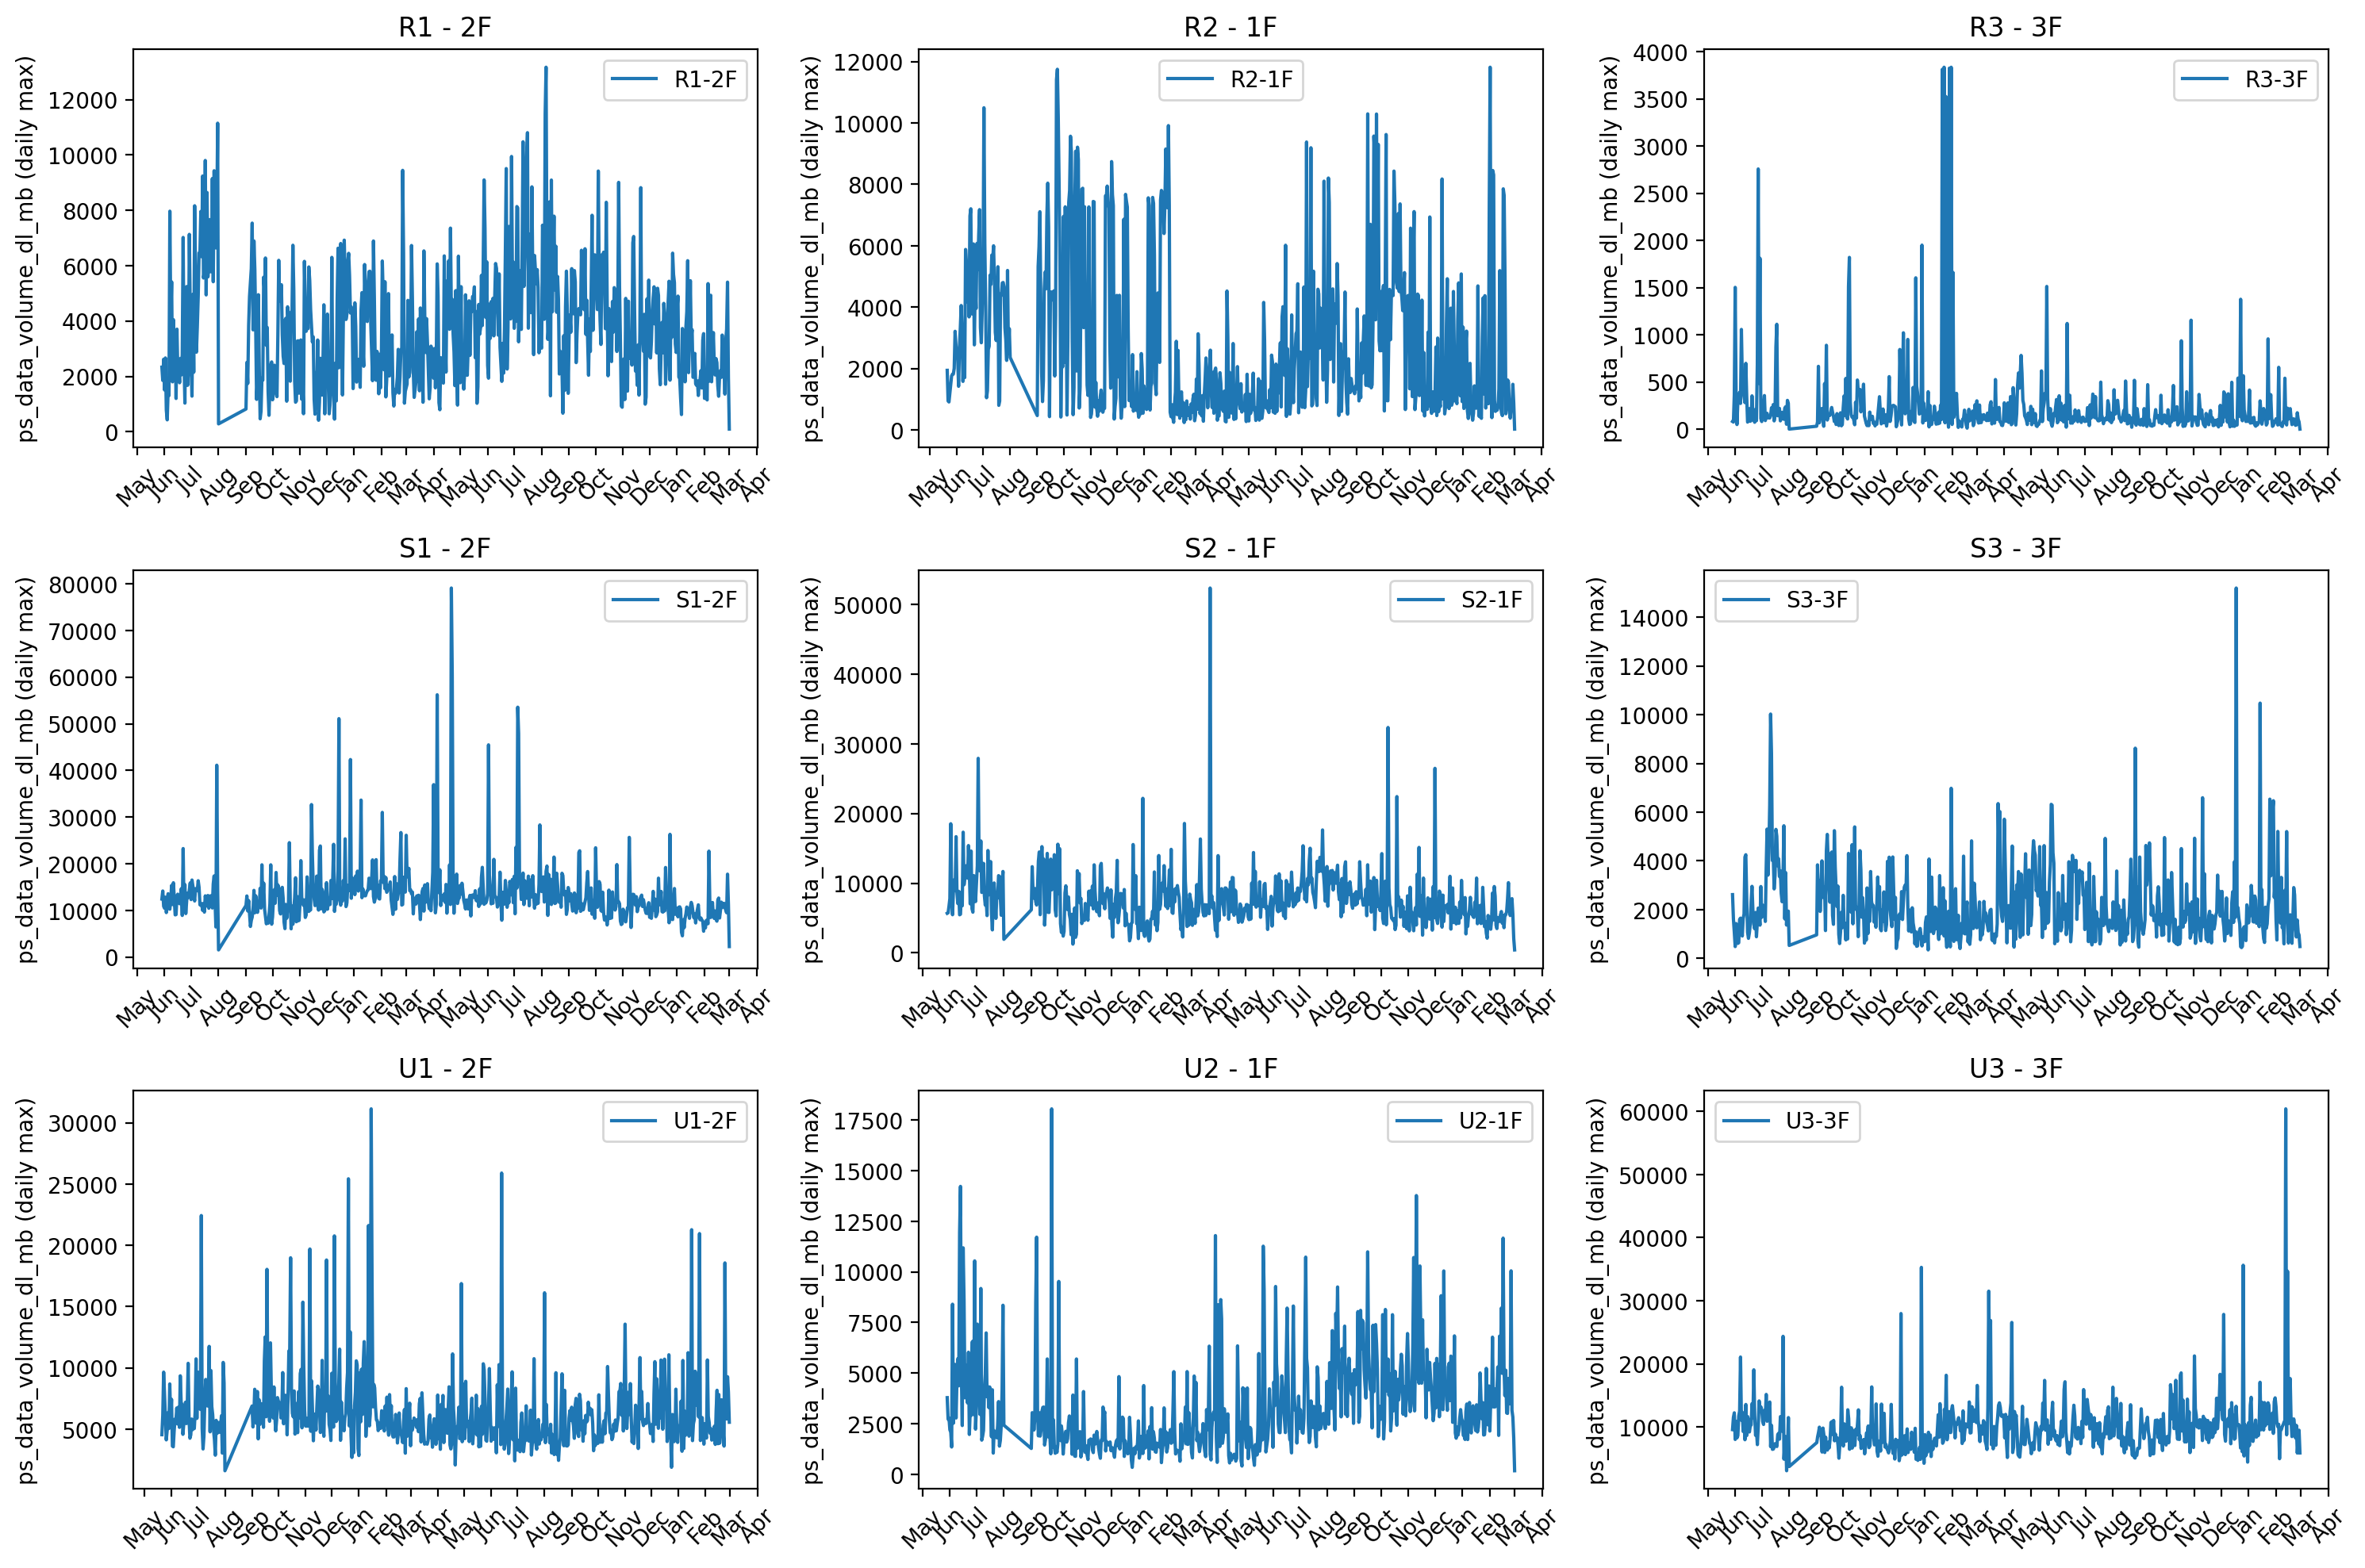
\includegraphics[width=\linewidth]{figures/9_tower_time_feature_daily_max.png}
    \caption{2F cell Daily peak data volume downlink across all sites}
    \label{fig:U1_vs_R1_daily_max}
\end{figure*}

To provide a clearer visualization of the dataset, Figure \ref{fig:U1_vs_R1_daily_max} shows the daily peak downlink data volume across all cells for two example towers, a recreational tower (R2) and an urban tower (U2). The figure also reveals a gap in August 2024 due to missing data in the dataset. \\

Already at this stage, clear differences in traffic behavior can be observed between the two tower types. The urban tower exhibits a relatively stable and gradually increasing trend over time, which suggests linear trend behavior. In contrast, the recreational tower displays strong seasonal variations, with traffic volumes increasing significantly during the summer months. These differences illustrate the differences in traffic volume across tower types and underscore the importance of treating each category separately in subsequent analysis. \\


\begin{figure}[H]
    \centering
    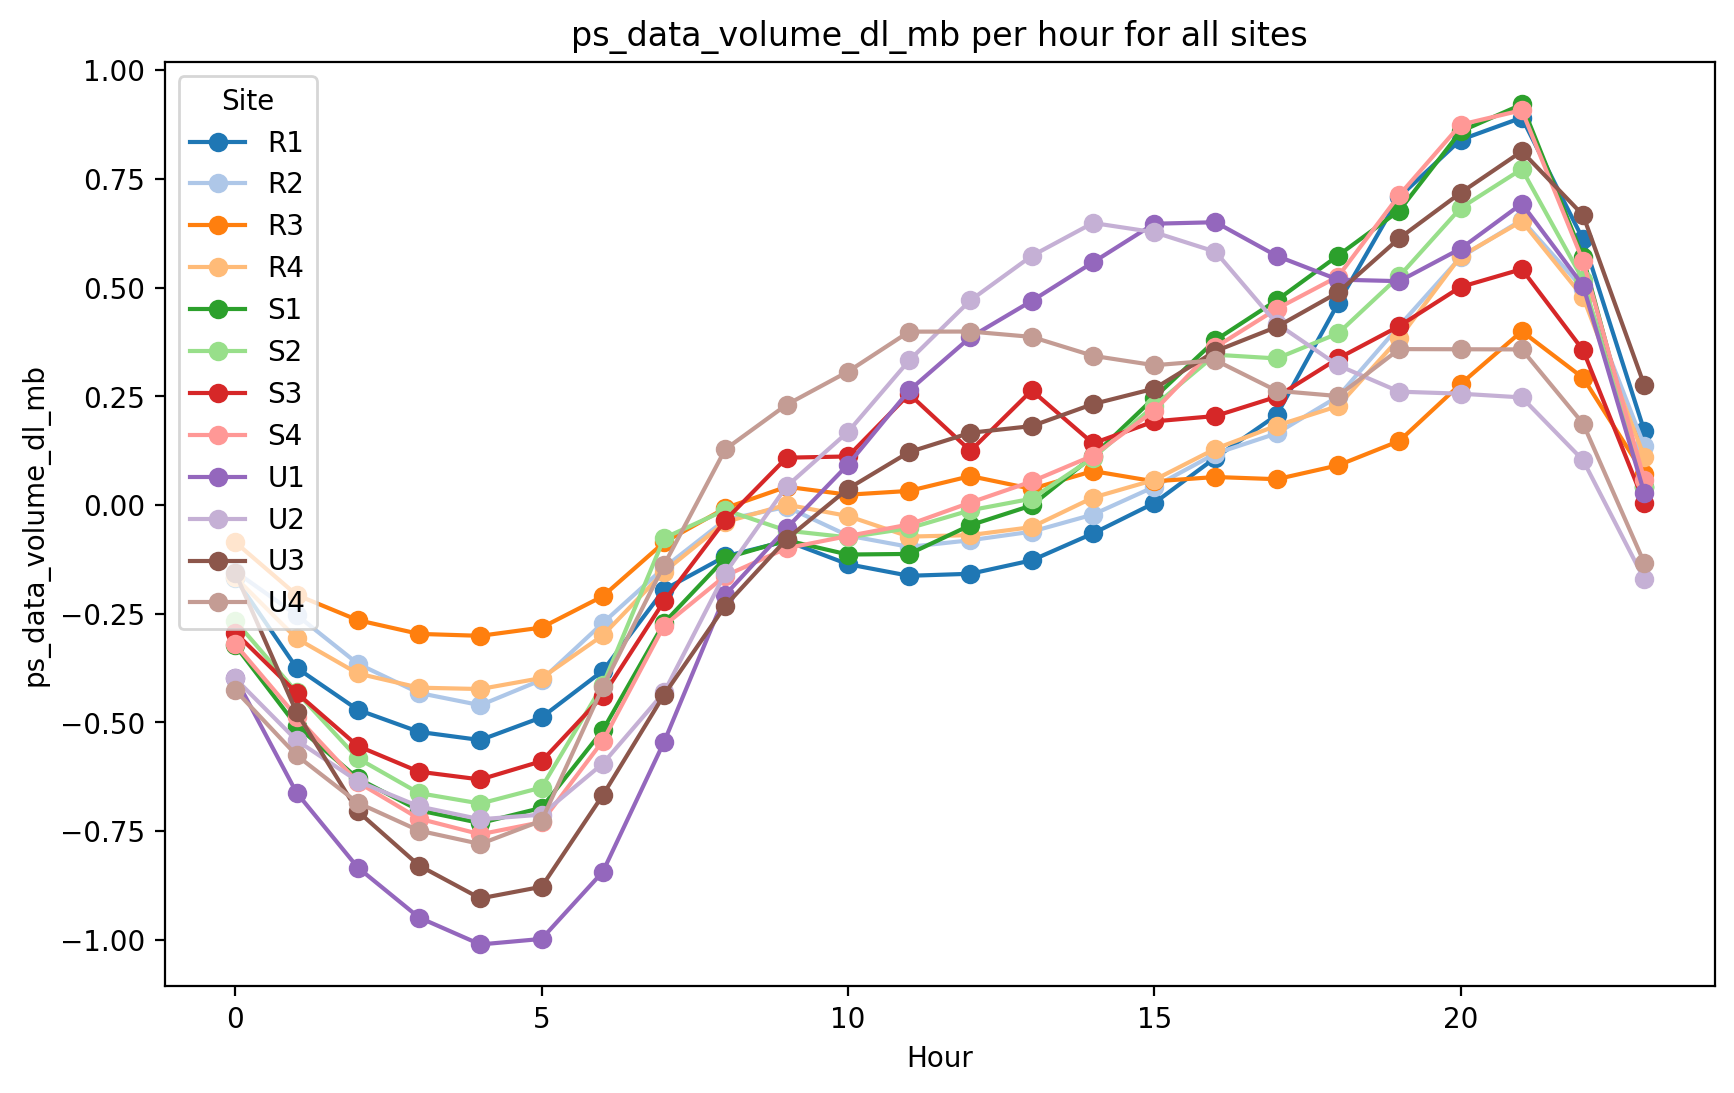
\includegraphics[width=\linewidth]{figures/avg_hourly_per_site.png}
    \caption{Average traffic volume per hour of day across all cells}
    \label{fig:avg_hourly_per_site}
\end{figure}

Figure \ref{fig:avg_hourly_per_site} shows the average hourly downlink data volume for each site, normalized using z-score standardization, to get a clear comparison in patterns across the sites. Clear differences can be seen between urban, suburban, and recreational cells. \\

All site types reach their minimum traffic between 03:00 and 05:00, with urban cells (U1--U4) showing the lowest values, with z-scores around (-0.75 to -1). This suggests that urban cells experience the strongest night-time drop relative to their average level, reflecting a clear difference between peak and off-peak demand in densely populated areas.. \\

Urban cells (U1-U4) recover quickly from the overnight minimum, reaching a mid day peaking around 11:00-16:00 at z-scores of approximately 0.5-0.65, and declining again after 16. Recreational cells (R1-R4) follow a different daily cycle, remaining 
relatively flat during midday near their mean (z-score $\approx$ 
-0.1 -- 0.1), before steadily increasing toward an evening peak 
around 20:00--21:00. Suburban cells (S1--S4) closely mirror this 
recreational pattern, with low daytime activity and a steady 
climb toward an evening peak, suggesting that both categories 
are driven by similar leisure and residential usage behaviour 
rather than the workplace and commuter patterns that dominate 
urban cells. \\

The most striking divergence occurs in the evening. Recreational and suburban cells reach their daily peak between 19:00 and 21:00, with several sites such as R1, S4, and S1 exceeding a z-score of 0.75. Urban cells also rise in the evening but peak slightly earlier, around 20:00, and at comparatively lower normalized levels. This represents an evening peak roughly 30--40\% higher in normalized terms than the midday plateau observed in urban cells, highlighting a fundamentally different daily usage cycle. \\

Notably, U3 and R2 deviate from the dominant patterns within their respective categories. U3 follows a pattern more similar to recreational sites, with low activity during the day and a pronounced evening peak around 20:00. \\




These results confirm that the timing of peak demand differs systematically by cell type. Urban cells follow a midday-dominated pattern consistent with workplace and commuter activity, while recreational and suburban cells follow an evening-dominated pattern more consistent with leisure usage. This distinction has direct implications for forecasting, as models trained on mixed cell types risk combining two structurally different daily cycles. \\

\begin{figure}[H]
    \centering 
    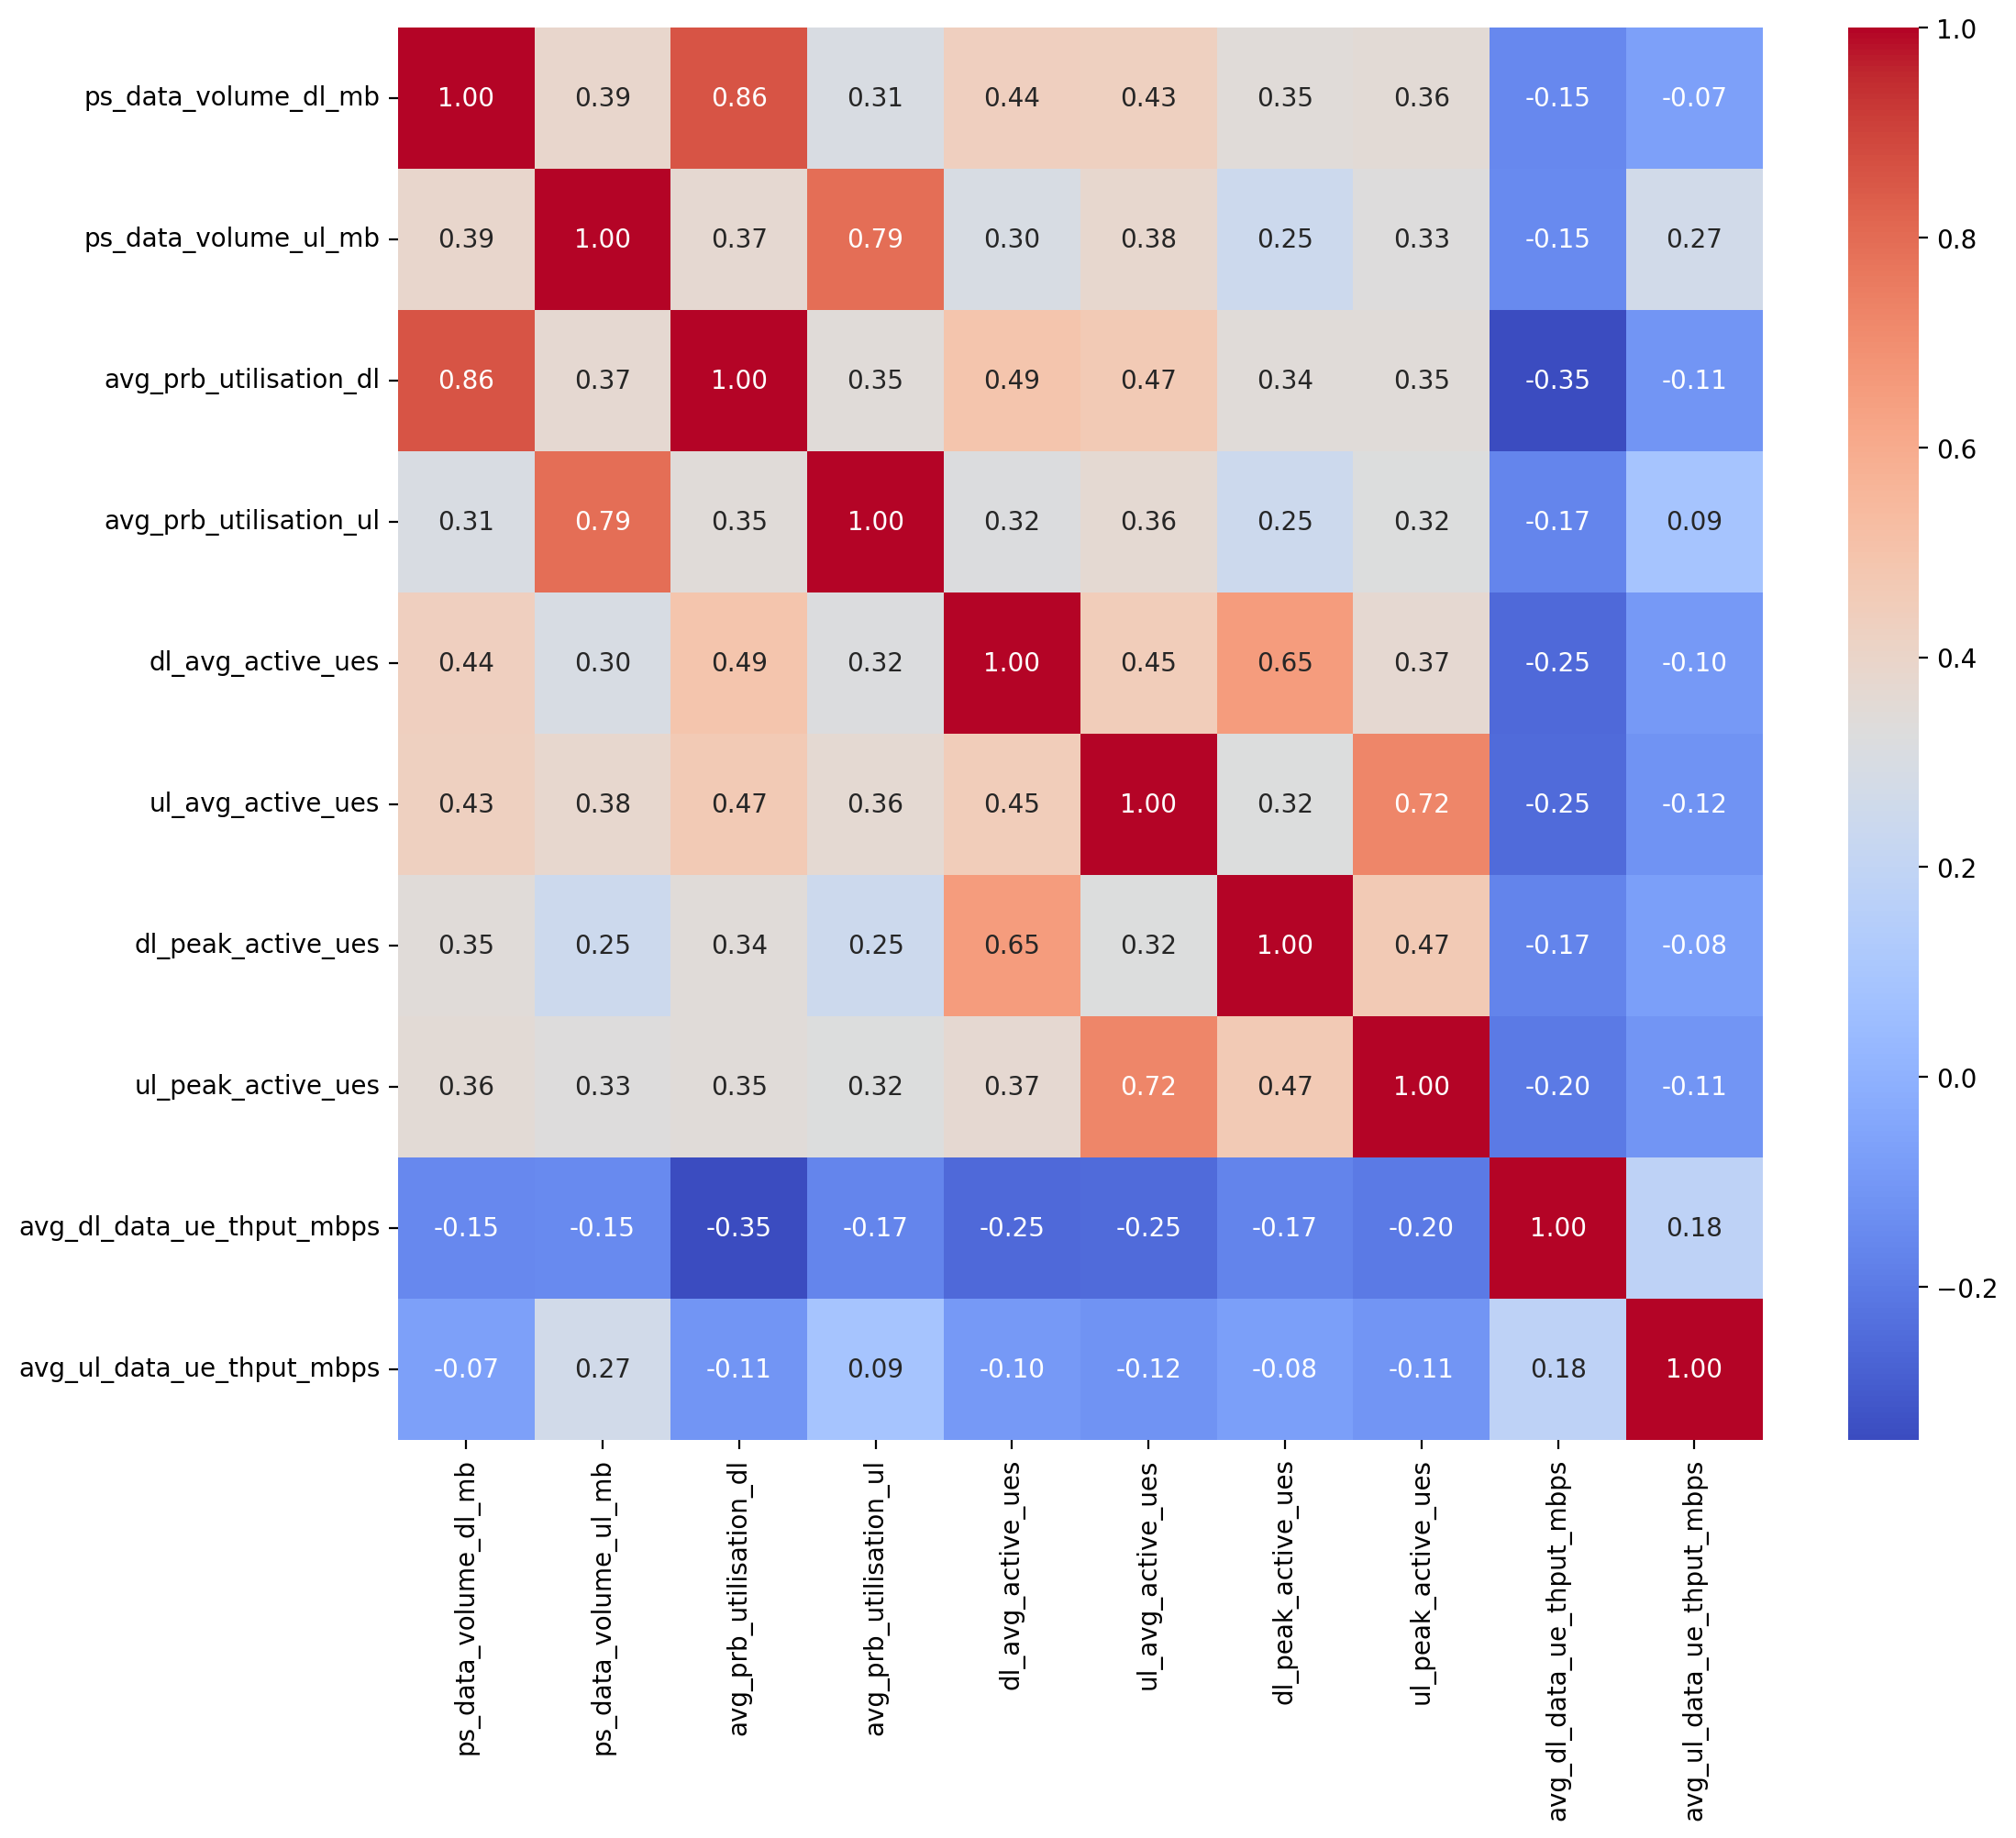
\includegraphics[width=\linewidth]{figures/correlation_matrix.png}
    \caption{Feature correlation matrix}
    \label{fig:correlation_matrix}
\end{figure}

Figure~\ref{fig:correlation_matrix} shows the correlation matrix of all continuous features in the dataset. Most features are positively correlated with each other. The main exception is user throughput (Mbps) negative correlations compared to the other features. \\

This behavior is expected. When a cell has fewer active users, it can allocate more throughput per user, which can lead to higher throughput values per user when overall traffic is low. \\

Data volume UL/DL and average PRB utilisation UL/DL are highly correlated at 0.86 for downlink and 0.79 for uplink. This is consistent with the theory presented in Section \ref{sec:resource_allocation}, more PRBs allocated generally means more data being transmitted. However, the correlation is not perfect, as poor radio conditions can force the scheduler to allocate more PRBs per unit of data, as illustrated in Figure \ref{fig:PRB_utilization}.

In general, features within the same category show strong correlations, such as average and peak values of the same feature. Another strongly correlated feature is the relationship between PS data volume and average PRB utilization, where higher traffic volume leads to higher resource usage in the cell. \\

Overall, the results suggest that traffic related metrics are strongly interdependent, meaning that a few key features, such as data volume, already provide a good representation of overall cell. \\
